% !TEX root =  ../FinalReport.tex

\chapter{Implementation}
\label{sec:Implementation}

Building the program was a huge technical challenge on many levels, resulting in 8.5k lines of code spread over 146 files in three different programming languages.
% involving three programming languages, % resulting in 8.5k lines of code built with three programming languages 
Solving the more complicated problems required some interesting tricks which may have interacted with lesser-known language features, memory models, and in one case the particulars of the C++17 specification.
The correctness of the resulting program was then ensured through the use of other features, including C++ macros and files that crossed language boundaries\footnote{See \cref{sec:Impl:Viz:CPUGPUSafety}.}.
This chapter documents these tricks and the background needed to understand them.

The first section contains an overview of relevant C++ features, and some other concepts employed while developing the program.
The next section focuses on Code Safety, detecting any faults during compilation and then ensuring any other faults do not then manifest into problematic errors.
As in the Design section, each layer of the codebase is then examined and all interesting problems solved during development are documented.

\section{Preliminary Work \& Background}
The primary languages used in the program are C++17 and CUDA.
This section will explain key elements of C++17 used in the program, the build system, and the external libraries used.

\subsection{C++ Primer}
Virtual classes use virtual functions to allow subclasses to override behaviour in the parent.
The seminal example is creating a parent class \texttt{Animal} which can \texttt{talk()}, and a subclass \texttt{Dog} which overrides \texttt{talk()} to bark. \todomark{Better example/code?}
When a virtual function is called on an object, instead of statically determining which function to call at compile-time, the \emph{vtable} of the object is read out at run-time with the correct function pointer.
In Java and Python all functions are considered virtual, but in C++ virtual behaviour can be selectively enabled.
As each virtual function call requires multiple indirections (object $\rightarrow$ vtable $\rightarrow$ function), the performance is slightly worse than using normal functions.
Virtual functions are avoided where possible in the codebase.
\todomark{Demo code https://godbolt.org/z/jYonzK76r}
\todocite{https://pabloariasal.github.io/2017/06/10/understanding-virtual-tables/}

C++'s largest innovation over C is the template system.
Classes and functions can be `templated' on types or values, and then `instantiated' when these parameters are known.
When such a class or function is instantiated a complete copy is created with the new parameter values, which is compiled and optimized separately from any other instantiations.
This is useful for encoding extra information in a type for safety, e.g. \mintinline{cpp}{VulkanShader<Vertex>} cannot be passed to a function expecting \mintinline{cpp}{VulkanShader<Compute>} because they're independent types.
It's also useful for static function dispatch, as instead of taking a virtual class with a \texttt{talk()} function you can instead template a function on the type of animal it uses, and call the function directly.
This technique is used in the Simulation to efficiently use Backends.
\todomark{https://godbolt.org/z/zz7jvTW6E template vfunc example}

\subsubsection{``Typeclasses''}
In other languages, like Haskell, a typeclass defines some behaviour a class should fit. From \todocite{Learn you a haskell}: ``If a type is a part of a typeclass, that means that it supports and implements the behavior the typeclass describes''.
C++17 does not have a convenient way of denoting this but it is especially helpful when building generic code with templates, as it allows the generic code to make assumptions about what behaviour types will support.
The rest of this chapter will define typeclasses where convenient to describe behaviour shared by certain classes.

\subsection{Build System}
The build system is implemented in CMake as specified in \cref{sec:ProjManagementTools}. %\cite{tool:Cmake}
This section highlights a few changes that were made to an otherwise standard setup to accommodate the project.

\subsubsection{CUDA-less Binaries}
The project can be built to produce both CUDA and CUDA-less binaries, in case it needs to be run on CUDA-less computers.
The list of regular C++ source files and CUDA source files are maintained separately. A CUDA-less binary (\shell{sim\_nocuda}) will only build the C++ files while a CUDA binary (\shell{sim\_cuda}) will build both.
When building the \shell{sim\_cuda} target the preprocessor macro \code{CUDA\_ENABLED} is defined throughout all source files, including the C++ files.
This allows support for CUDA backends in C++ code (i.e. as selectable options on the command-line) to be conditionally enabled without maintaining two copies of the relevant source files.
In \cref{fig:ConditionalCUDA} (which has been amended for brevity), the switch statement only contains a case for CUDA if the directive is set, triggering a fatal error otherwise.
\begin{figure}[ht]
    \centering
\begin{cppcode}
switch(backendType) {
    case Null:
        return SimFixedTimeRunner<NullSimulation, Host2DAllocator>();
    case CpuSimple:
        return SimFixedTimeRunner<CpuSimpleSimBackend, Host2DAllocator>();
    case CpuOptimized:
        return SimFixedTimeRunner<CpuOptimizedSimBackend, Host2DAllocator>();
    case CpuAdapted:
        return SimFixedTimeRunner<CpuOptimizedAdaptedSimBackend, Host2DAllocator>();
#if CUDA_ENABLED
    case CUDA:
        return SimFixedTimeRunner<CudaBackendV1<true>, CudaUnified2DAllocator>();
#endif
    default:
        FATAL_ERROR("Enum val %d doesn't have an ISimFixedTimeRunner!\n", backendType);
}\end{cppcode}
\caption{Conditionally supporting CUDA based on a preprocessor directive}
    \label{fig:ConditionalCUDA}
\end{figure}


% \todomark{Move Shader Build Infrastructure somewhere else?}
\subsubsection{Shader Build Infrastructure} % Fits in with the build system vibe
The shaders used for visualization are written in GLSL, with appropriate extensions to be compatible with Vulkan.
They are separated by file type, with Vertex shaders in \shell{.vert} files and Fragment shaders in \shell{.frag} files.
As Vulkan does not natively support GLSL, they must be compiled to SPIR-V before they can be used.
CMake does not support GLSL as a first-class language, so a custom build command was used to compile them with \shell{glslc}\cite{GoogleLLCShaderc} when they change.
This allows them to be treated just like any other source file from the programmer's perspective.
The SPIR-V files are placed in a \shell{shaders} directory next to the binaries, where they can be easily accessed and passed to Vulkan.

% \todomark{Code Safety - emphasis on using templates, compile-time checks, and failing that runtime assertions.}

\subsection{Library Selection}
\label{sec:LibrarySelection}
\begin{figure}[ht]
    \centering
    \begin{tabular}{r|c c}
        & OpenGL & Vulkan \\
        \hline
        OpenCL & Y & N \\ 
        CUDA & Y & Y \\ 
        OpenGL & Y & N \\ 
        Vulkan & N & Y \\ 
    \end{tabular}
    \caption{Graphics and Compute Backend Interoperability Matrix}
    \label{fig:LibraryChoices}
\end{figure}
CUDA and Vulkan have been chosen as backends, but other backends were also considered.
As the simulation would have to run on DCS systems (\cref{reqN:DCSCompile}) and thus run on Linux, the only possible GPU rendering backends were OpenGL and Vulkan.
However, there were still multiple choices of compute backend:
\begin{itemize}
    \item OpenCL\cite{tool:OpenCL1.0PressRelease} is an ``Open Standard for Parallel Programming of Heterogeneous Systems''\cite{TheKhronosGroupOpenCLInc}.
    \item CUDA\cite{tool:CUDA} is a closed-source library for running parallel code on NVIDIA GPUs.
    \item OpenGL has Compute Shaders\cite{tool:OpenGLComputeShaderExt} which can execute computations outside of the graphics pipeline.
    \item Vulkan also has Compute capability\cite{TheKhronosGroupVulkanGuide}, similar in function to OpenGL.
\end{itemize}
To decide on the compute backend to use, an interoperability matrix was drawn (\cref{fig:LibraryChoices}) to show which libraries could share data without copying it between buffers.
As the researcher was already experienced with Vulkan, and the more granular control it provides would be beneficial to performance, Vulkan was selected as the rendering backend.
This prevented OpenCL and OpenGL from being used as compute backends, as they are not compatible with Vulkan.
CUDA and Vulkan have comparable ability, but CUDA was chosen as the compute backend.
The Vulkan compute shaders are still a very graphics-oriented view of computation, and CUDA would give the researcher experience with other kinds of libraries.
A Vulkan compute backend is used for the visualization portion of the code.

% Not for now, but note that the C++ vulkan bindings are nice. They do end up wrapped in other classes, but they remove the need to remember boilerplate as much.

In other cases, there were clear choices: the SDL2\cite{SimpleHomepage} window and input library and the Dear ImGUI\cite{CornutDearImGui} UI library were chosen due to personal experience.
The \shell{stb\_image.h} header was found to be a simple method of importing image colour data as byte arrays, used for the input generator (\cref{req:GenerateState}).

There are a great many options for Command-Line parsing libraries, even more so because C++ is used instead of C.
A recent survey of the possibilities\cite{attractivechaos2018AC/C++} was whittled down to five options.

\code{getopt}\cite{FreeSoftwareFoundationGetopt3:Page}, \code{argp}\cite{GNUProjectArgpLibrary}, and \code{gopt}\cite{VajzovicGoptLibrary} are C libraries that use arrays of structures to define the required arguments.
Of them, only \code{argp} can automatically generate a \shell{--help} argument, which is a very valuable feature.
\code{cxxopts}\cite{jarro2783Cxxopts:Parser} was considered as a C++ alternative but used very odd syntax for defining arguments.
Ultimately CLI11\cite{CLIUtilsCLI11} was chosen as a modern C++11 library that had native support for subcommands, which were used heavily for separating program components (see \cref{sec:DesignSubcommands}).

% \todomark{Resource Management}
\pagebreak
\section{Code Safety}\label{sec:Impl:CodeSafety}
No program is faultless, and when faults manifest during execution it's important to ensure they have a minimal effect on their surroundings.
This program includes many means of detecting errors both at compile-time and run-time to ensure its dependability.

The G++ flag \shell{-Wall} enables many warnings that are emitted at compile-time if potential errors are detected.
Unlike some other languages (i.e. Verilog) these warnings are generally reliable and it is feasible to build a C++ program that compiles without any warnings.
To ensure this the \shell{-Werror} flag is added to upgrade these warnings to compilation errors, ensuring a program which compiles will be warning-free\footnote{Some warnings, such as those from \shell{-Wextra} and those relating to unused variables and parameters, are usually benign so weren't upgraded.}.

Runtime errors are detected with a set of C++ macros that check if required conditions are met.
As there is no liveness requirement for the program, failure triggers an immediate program exit to avoid errors propagating through the system.
The \code{DASSERT} family of macros are included only in Debug builds, and the \code{FATAL\_ERROR} family of macros test both in Release and Debug.
Both families print a message including the file and line of code that triggered the error, and any other relevant debug information.
These families are also integrated with the \code{CHECKED\_CUDA} and \code{CHECKED\_VULKAN} macro families, which surround CUDA/Vulkan function calls and check the returned error codes.
An example is shown in \cref{fig:ImplAssertions}.
\begin{figure}[t]
    \centering
    \begin{subfigure}{0.49\textwidth}
        \begin{minted}{cpp}
if (value == unexpected) {
    FATAL_ERROR(
        "Unexpected Value %d\n",
        value
    );
}
// equivalent to
FATAL_ERROR_IF(
    value == unexpected,
    ...
);
// or
FATAL_ERROR_UNLESS(
    value != unexpected,
    ...
);

// Same, but only fails in Debug builds
DASSERT(value != unexpected);
        \end{minted}
        \caption{Example of assertion macros}
    \end{subfigure}%
    \begin{subfigure}{0.49\textwidth}
        \begin{minted}{cpp}
cudaError_t error = cudaDeviceSynchronize();
FATAL_ERROR_IF(error != cudaSuccess);
// Equivalent to
CHECKED_CUDA(cudaDeviceSynchronize());

auto result = vkDeviceWaitIdle();
FATAL_ERROR_IF(result != vk::Result::eSuccess);
// Equivalent to
CHECKED_VULKAN(vkDeviceWaitIdle());
        \end{minted}
        \caption{Example of API failure safety macros}
    \end{subfigure}
    \caption{Examples of error safety via macros}
    \label{fig:ImplAssertions}
\end{figure}

The final tool for error detection is the Vulkan Validation Layer.
This is a standard Vulkan extension which checks each Vulkan call to ensure the Vulkan specification \cite{TheKhronosGroupVulkanSpec} isn't violated.
These checks are very in-depth, and are a must-have when debugging visualization errors.
The base Vulkan functions don't do this error checking for efficiency's sake, and the program disables these layers in Release mode for the same reason.

\subsection{Smart Resource Classes}
All memory allocations, CUDA objects, and Vulkan objects follow the same allocate/release pattern.
They are not destroyed automatically when they go out of scope, but must be released manually.
This is an error-prone process, as a programmer may forget which resources need to be released or try to release a resource twice.

\begin{figure}
    \centering
    \begin{cppcode}
// Manual handling
{
    auto* semaphore = new Semaphore();
    // do things with semaphore...
    delete semaphore;
}

// Automatic handling
{
    std::unique_ptr<Semaphore> semaphore = std::make_unique<Semaphore>();
    // do things with semaphore...
    // automatically deleted
}
    \end{cppcode}
    \caption{Example of memory management with C++ standard classes}
    \label{fig:ImplUniquePtr}
\end{figure}

Smart resource classes alleviate this by tying the resource lifetime to a C++ object, using the object \emph{destructor} to release the resource.
The prime example of this is \code{std::unique_ptr<T>}, which holds a \code{T*} object and \code{free()}-s it when the object leaves scope (\cref{fig:ImplUniquePtr}).
However this does not easily map to other deletion methods, and the pointer adds an unwanted extra level of indirection.
\code{vulkan.hpp}, included in the Vulkan SDK, includes similar classes for each type of Vulkan resource, but still requires a lot of boilerplate to initially create objects\footnote{Vulkan objects require a full CreateInfo struct to create, rather than taking function arguments.}.
In some cases, it's also more convenient to store multiple resources together, such as a buffer and the device memory it uses, which cannot be directly achieved with either method.
To solve these problems custom smart resource classes are implemented for individual resources and aggregates, with more convenient constructors (see \cref{sec:appx_resourceclasses}).

These smart classes are affected by C++ copy/move semantics.
C++ allows objects to be copied with a copy-constructor, or moved with a move-constructor.
The resource objects should not be copyable as it would become unclear which copy would be responsible for destroying the resource.
The copy-constructor can be deleted to prevent this, but the move-constructor is useful for transferring ownership e.g. from a resource factory to the person using the resource.

When an object is moved, the original version should forget the data it's holding and give it to the new object.
C++ can generate this constructor automatically, but this ``default move-constructor'' will just copy the data across if the data is \textit{TriviallyCopyable}\cite{cpprefMoveConstructor}.
%, and is true for pointers and all CUDA handles.
All pointers and CUDA handles are \textit{TriviallyCopyable}, so they don't get forgotten automatically.
Manually writing each move-constructor to address this would be error-prone, so instead the \code{ForgetOnMove<T>} class is used to wrap these values and automatically forget them when the move-constructor is invoked.
% To avoid manually creating move-constructors, which is error-prone, the \code{ForgetOnMove<T>} class wraps these values and automatically forgets them when the move-constructor is invoked.
The final result is shown in \cref{fig:ForgetOnMoveEx}: a clean, easy, and safe method of implementing new smart resource classes.
% Detecting and mitigating these faults and errors is an important part of effective programming, 
\begin{figurepage}
\begin{figure}
    \centering
    \begin{cppcode}
// Doesn't use ForgetOnMove<>
class ComplexWrapper {
    void* memoryPointer;
    
    // Constructor
    ComplexWrapper(size_t memorySize) {
        // Allocate memory
    }
    // Destructor
    ~ComplexWrapper() {
        if (memoryPointer != nullptr) {
            // Free memory
        }
    }
    
    // Copy constructor - deleted
    ComplexWrapper(const ComplexWrapper&) = delete;
    // Move constructor - complicated
    ComplexWrapper(ComplexWrapper&& movedFrom) {
        this->memoryPointer = movedFrom.memoryPointer;
        movedFrom.memoryPointer = nullptr;
    }
};

// Uses ForgetOnMove<>, is simpler
class SimpleWrapper {
    ForgetOnMove<void*> memoryPointer;
    
    // Constructor as before
    SimpleWrapper(size_t memorySize) {
        // Allocate memory
    }
    // Destructor as before, but checks if the memoryPointer is present
    ~SimpleWrapper() {
        if (memoryPointer.has_value()) {
            // Free memory
        }
    }
    
    // Copy constructor - deleted
    SimpleWrapper(const SimpleWrapper&) = delete;
    // Move constructor - defaulted!
    // We don't have to write this in full
    SimpleWrapper(SimpleWrapper&&) = default;
};
    \end{cppcode}
    % \caption{Example of \code{ForgetOnMove<T>} vs. manual handling.}
    % \caption{Comparing \code{ForgetOnMove<T>} to manual handling.}
    \caption{Automatic forgetting with \code{ForgetOnMove<T>} vs. manual handling}
    \label{fig:ForgetOnMoveEx}
\end{figure}
\end{figurepage}

\pagebreak
\section{Memory Layer}
As mentioned in the Design section, all elements of the Memory system are parameterized on the memory type.
This was accomplished by creating an enum \code{MType} and a set of classes templated on it (\cref{fig:TypeclassMemory}).
These templates were then specialized for each type of memory, implementing the logic for each type separately.
Separate implementations were required due to the unique constraints and allocation methods of each memory type.

\begin{figure}
    \centering
\begin{minted}{cpp}
enum MType {
    CPU,
    Cuda,
    VulkanCuda
};

enum RedBlackStorage {
    RedBlackOnly, // Just store the red and black matrices
    WithJoined // Store the red, black, and combined matrices
};

typeclass DataArray {
    // Has a static value MemType telling you what memory type it takes
    static MType MemType;
    // Has a function for calculating the total bytes used for a matrix
    static size_t sizeBytesOf(Size<uint32_t> size);
}

typeclass FrameAllocator<MType> {
    // Function for allocating a 2D array
    Sim2DArray<T, MType> allocate2D(Size);
    
    // Function for allocating a red/black array
    SimRedBlackArray<T, MType, RedBlackStorage> allocateRedBlack(Size);
}

typeclass FrameSetAllocator<MType, TFrame> {
    std::vector<TFrame> frames;
}
\end{minted}
    \caption{Memory Layer Typeclasses}
    \label{fig:TypeclassMemory}
\end{figure}

\subsection{Array Handles}
The \code{Sim2DArray<T, MType>} and \code{SimRedBlackArray<T, MType, RedBlackStorage>} classes represent handles to 2D arrays of values of type \code{T}.
They implement a common \emph{DataArray} typeclass (\cref{fig:TypeclassMemory}).
They do not own the data they point to, so if a \code{Sim2DArray} is destroyed the referenced memory isn't freed.
Freeing memory is handled by the \code{FrameAllocator} instead.

\code{SimRedBlackArray} serves as an aggregate of \code{Sim2DArray}s, without defining any special behaviour.
It does not specialize on the memory type, but provides two storage variants \code{RedBlackOnly} and \code{WithJoined} (\cref{fig:TypeclassMemory}).

\code{Sim2DArray} implements a set of functions for accessing data from the CPU, CUDA, and Vulkan.%GPU, and as Vulkan handles.
These functions are only present if that access type is supported, so trying to use an unsupported function results in a compile-time error.
Other more generic operations are also supported such as zeroing out memory, copying memory in from different sources, and copying memory out to the CPU.
Each of these is implemented differently based on the memory type, and may not be implemented if the operation is impossible.
For example attempting to `prefetch', i.e. move CUDA Unified Memory to the GPU, is only supported for CUDA Unified Memory and not the other types.
% \todomark{Matrix of supported operations}

\subsection{\texttt{FrameAllocator}}
\code{FrameAllocator<MType>} is an allocator associated with a single memory frame.
The behaviour is specialized for each memory type, but each specialization fits a typeclass (\cref{fig:TypeclassMemory}) for allocating 2D and red-black arrays.
The \code{FrameAllocator} owns these allocations, and when it is destroyed the allocations are freed.
The CPU and CUDA Managed memory variants allocate data directly using their respective allocation functions when requested, store the raw pointers in a list, and frees all of them on destruction.

The Vulkan variant allocates a fixed amount of Vulkan device memory, which is exported using the CUDA-Vulkan interop API to a CUDA-compatible pointer.
All new allocations are then sub-allocated from this memory.
The fixed amount is calculated by the \code{FrameSetAllocator}, which assumes only the bare minimum ($u, v, p, fluidmask$) requirements are allocated in Vulkan.
The associated CUDA pointer is \emph{not} compatible with Unified Memory, so cannot be paged to the CPU.

\subsection{\texttt{FrameSetAllocator}}
\code{FrameSetAllocator<MType, TFrame>} creates a set of TFrame objects which are each allocated using separate \code{FrameAllocator<MType>} objects.
The CPU and CUDA variants simply construct N \code{TFrame}s using N \code{FrameAllocator}s.
The Vulkan variant is more advanced as it has to check the \code{TFrame} exposes the correct data, calculate the amount of Vulkan data to allocate per frame, and expose this data by implementing a virtual \code{VulkanFrameSetAllocator} interface.
The Vulkan variant also passes in a CUDA \code{FrameAllocator} with the Vulkan one to allow the other buffers to be allocated.

\subsection{Usage in Other Layers}
The Simulation layer instantiates \code{FrameSetAllocator}s in the simulation Runners.
The Backend typeclass (\cref{fig:TypeclassBackend}) requires each backend to implement a Frame class, and to take a list of Frame instances as an argument to their constructor.

The visualization uses the \code{VulkanFrameSetAllocator} interface to grab references to simulation memory, which it uses while rendering. %and use these references while rendering.


\pagebreak
\section{Simulation Layer}
As shown in the Design section, the Simulation layer is split into generic Runners and multiple simulation Backends.
% Building a system that efficiently allowed Runners to be Backend-agnostic and still performance was nontrivial.
Building a system that efficiently allowed Runners to be Backend-agnostic while remaining performant was nontrivial.

\subsection{Runners}
Runners had three major design constraints:
\begin{enumerate}
    \item Runners should be generic with respect to the backends they implement.
    \item The same Runner should have the same interface for each Backend it implements.
    \item Virtual functions should be avoided where possible.
\end{enumerate}
The immediate thought would be to implement a single Runner class, taking a virtual Backend class and using virtual functions to start each tick.
This would meet (1) by using a virtual Backend interface, and (2) by using the same class for all Backends, but would violate (3) by forcing every Backend to use virtual function calls.
Instead, a slightly more complex approach is taken.

Each Runner defines a virtual interface, such as \code{IFixedTimeRunner} for the fixed time runner.
A templated implementation class \code{SimFixedTimeRunner<B>} is then instantiated for each compatible backend \code{B}.
% A templated implementation class is then instantiated for each compatible backend, such as \code{SimFixedTimeRunner<CpuBackend>}, \code{SimFixedTimeRunner<CUDABackendV1>}, etc.
Each of these classes implements the virtual interface \code{IFixedTimeRunner}, but they call the simulation functions directly as they are templated on the backend type.
This setup meets (1) by using a single templated implementation, (2) by implementing a virtual interface, and (3) by only using the virtual functions where absolutely necessary i.e. on the Runner itself.
This allows \code{IFixedTimeRunner} implementations to define a single virtual function \code{runForTime(t)} instead of calling a virtual function every simulation tick.

\subsection{Backends}
To allow the generic implementation described above, the Backend typeclass ensures all backends follow a consistent interface (\cref{fig:TypeclassBackend}).
Five classes implement this typeclass, matching those described in \cref{sec:DesignBackends}:
\begin{itemize}
    \item \code{NullSimulation}
    \item \code{CPUSimpleSimBackend}
    \item \code{CPUOptimizedSimBackend}
    \item \code{CPUOptimizedAdaptedSimBackend}
    \item \code{CudaBackendV1}
\end{itemize}
% Aside from the trivial Null Simulation, these can be split into CPU and CUDA-based backends.

\begin{figure}
    \centering
\begin{cppcode}
typeclass BackendFrame {
    // Must have a constructor that takes an allocator
    BackendFrame(FrameAllocator<MemoryType> allocator);
}
typeclass Backend {
    // Must define a Frame class
    class Frame fits BackendFrame;
    // Must have a constructor
    Backend(std::vector<Frames>, FluidProperties, SimSnapshot);
    
    float findMaxTimestep();
    void tick(float timestep, int targetFrame);
    
    LegacySimDump dumpStateAsLegacy();
    SimSnapshot get_snapshot();
}    
\end{cppcode}
    \caption{Backend typeclass}
    \label{fig:TypeclassBackend}
\end{figure}

\subsubsection{CPU Backends}
Most of the simulation code for CPU backends has been directly copied from the original simulation\cite{modules:CS257Coursework}\cite{modules:aca257submission}.
Some templates and template specializations have been added for the Adapted backend, but for the most part, the simulation is unchanged.
The backend classes simply wrap up this code to be compatible with the typeclass.

\subsubsection{CUDA Backend}
The CUDA backend is where the bulk of new simulation work has been done.
As stated in the Design section, all simulation code has been ported to CUDA Kernels.
Each of these kernels takes a \code{CommonParams} struct as the first argument, containing run-time constants such as the simulation grid size.
To ensure \code{const __restrict__} pointers are used wherever possible, all other kernel arguments must be either an \code{in_matrix<T>} or an \code{out_matrix<T>}.
These templates alias to simple pointers which properly use \code{const} and \code{__restrict__} (\cref{fig:ImplMatrices}).
Using these enforces that each kernel has clear, distinct inputs and outputs, and that the inputs are read from fast global memory.

\begin{figure}[t]
    \centering
    \begin{subfigure}{0.49\textwidth}
        \begin{minted}{cpp}
template<typename T>
using in_matrix = 
    const T* const __restrict__;

template<typename T>
using out_matrix = 
    T* const __restrict__;
        \end{minted}
        \caption{Matrix templates}
    \end{subfigure}%
    \begin{subfigure}{0.49\textwidth}
        \begin{minted}{cuda}
__global__ void computationKernel(
    CommonParams config,
    in_matrix<float> inputs1,
    in_matrix<int> inputs2,
    
    out_matrix<float> output
);
        \end{minted}
        \caption{A kernel using the matrix templates}
    \end{subfigure}
    \caption{Example of CUDA matrix templates}
    \label{fig:ImplMatrices}
\end{figure}

The most intensive step in every implementation is the Poisson iterations, which are individually trivial but intensive at scale.
During development the profiler showed large gaps between the individual kernel runs, equivalent to almost 50\% of the runtime.
Each kernel was finishing quicker than the CPU could enqueue a new one, so to solve this a CUDA Graph was employed.
CUDA Graphs consist of a prerecorded set of kernel invocations with constant arguments.
A CUDA Graph was recorded that consisted of 100 Poisson kernels, and this was launched instead of the individual kernels.
This resulted in a 2x speedup in the profiler (see \cref{fig:CudaGraphsImpact}), but almost no speedup in practice.
The CPU overhead for each enqueue may be larger in the profiler, which would explain why this behaviour is not present in the final simulation.

The timestep calculation is implemented with two reductions, based on the second kernel from \cite{CUDAParallelReduction}\footnote{This isn't the fastest kernel, but reductions aren't frequent enough for it to matter.}.
A constant factor N is chosen, and the values in the array are reduced by a factor of N multiple times until only one is left.
Two data buffers are used to ping-pong the reductions - each iteration flips the input and output, so data is reduced from A to B to A and so on.

Because there are two reductions, it is most efficient to perform the first one asynchronously and enqueue both before waiting for them to finish.
By default copying reduction results back to the CPU is synchronous, which prevents this.
Allocating pinned memory, which cannot be paged to disk or moved around by the OS, allows the copy to be done asynchronously.

\begin{figure}
    \centering
    \begin{subfigure}{\textwidth}
        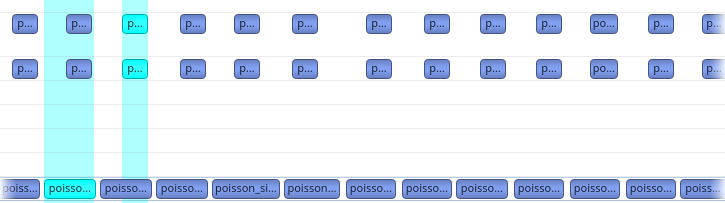
\includegraphics[width=\textwidth]{Ch48Implementation/figures/cudagraphs_before.png}
        \caption{Before CUDA Graphs}
    \end{subfigure}
    \vspace{1cm}
    \begin{subfigure}{\textwidth}
        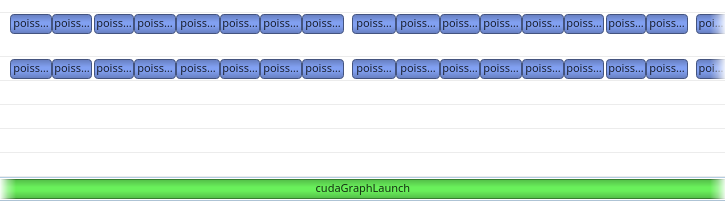
\includegraphics[width=\textwidth]{Ch48Implementation/figures/cudagraphs_after.png}
        \caption{After CUDA Graphs}
    \end{subfigure}
    \caption{Profiler traces of the Poisson kernels before and after CUDA graphs}
    \label{fig:CudaGraphsImpact}
\end{figure}

\begin{figure}
    \centering
    \begin{subfigure}{0.49\linewidth}%
        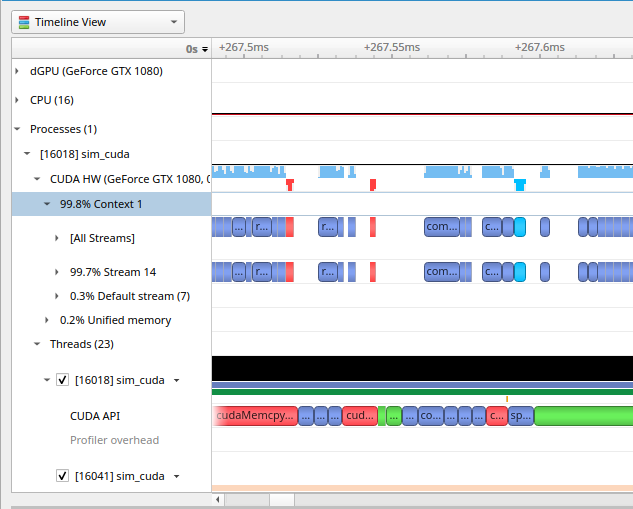
\includegraphics[width=\linewidth]{Ch48Implementation/figures/memcpy_sync.png}%
        \caption{Synchronous Copy}%
    \end{subfigure}%
    \begin{subfigure}{0.49\linewidth}%
        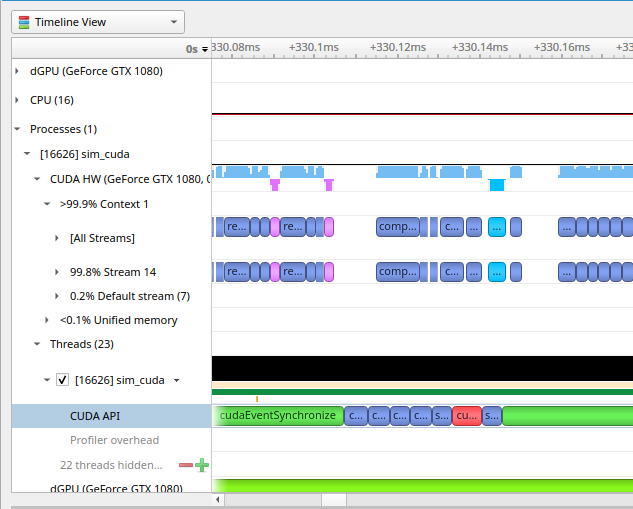
\includegraphics[width=\linewidth]{Ch48Implementation/figures/memcpy_async.png}%
        \caption{Asynchronous Copy}%
    \end{subfigure}
    \caption{Using asynchronous copies for greater efficiency}
    \label{fig:async_copy}
\end{figure}

% Copying the result back to the CPU is done asynchronously, which requires pinned memory to be allocated\todocite{pinned memory}.
% Normal virtual memory can be paged to disk or moved around by the OS, which means there is no reliable location for the GPU to eventually copy data to.
% Pinned memory must be specially allocated, and cannot be moved around, so the asynchronous copy can go ahead as planned.
% If pinned memory were not used the copy to CPU would be synchronous, which would delay the second 

% The profiler showed X when not using pinned memory, as copies to non-pinned CPU memory are synchronous so must wait for the first reduction before enqueueing the second.

% Currently the CUDA program uses the second kernel model, and this is planned to be moved up to the seventh kernel in the future.

% The CUDA program uses the second kernel model. 
% Upgrading to the seventh model was considered, but as the program does not include the residual check, the reductions are infrequent enough (two per tick) that upgrading was not necessary.
% In the future, this may be improved if Poisson residuals were introduced.\todomark{actual future work}
% \todomark{Mention pinned memory here}

\subsection{Usage in Other Layers}
The visualization layer instantiates a \code{VulkanTickedRunner} with \code{CudaBackendV1} to run a visualized simulation.

The command-line layer instantiates a \code{FixedTimeRunner} with any one of the backends to run a headless simulation.

\pagebreak
\section{Visualization Layer}\label{sec:ImplementationViz}
\subsection{Multithreading}
The worker thread is implemented with a \mintinline{cpp}{SystemWorker} class combined with a generic threading system.
% While only one worker thread is ever used in the final program, earlier versions planned to use a few unique workers so a generic system was required.
An \mintinline{cpp}{IWorkerThread} virtual interface is defined and \mintinline{cpp}{IWorkerThread_Impl<Worker>} implements this for a specific \mintinline{cpp}{Worker} class, similar to the Simulation Runners pattern.
% A similar pattern to Simulation Runners is used, where an \mintinline{cpp}{IWorkerThread} virtual interface is defined and a \mintinline{cpp}{IWorkerThread\_Impl<Worker>} class implements this for a specific \mintinline{cpp}{Worker} class.

% The \mintinline{cpp}{IWorkerThread} class works with a \mintinline{cpp}{WorkerThreadController} class.
To kick off the worker thread, a \mintinline{cpp}{WorkerThreadController} writes to a mutex-protected set of input data.
The `work index' of this data is incremented to signal it is new, and a condition variable is signalled to alert the worker thread and begin processing.
Work cannot be enqueued until the thread produces an output, which is sent to the main thread in the same way as before - a mutex is taken to update the output data with the new index, and the condition variable is signalled in case the main thread is waiting for the worker to finish.

\subsection{GPU Work Breakdown}
% \todoref{GPU work breakdown design} showed a coarse breakdown of work between the Viz Compute and Viz Graphics stages, which \cref{fig:VizDataTransform} expands on.
\cref{fig:VizDataTransform} expands on the coarse GPU work breakdown from \cref{sec:Design:Viz:Breakdown}.
Each rectangle represents a piece of memory, and each arrow represents a transformation from input to output via a compute shader, an image layout transfer, or a graphics pipeline.
Most memory is global rather than per-frame, as the system does not run any visualization stages in parallel.
Some per-frame memory is used to allow race-free accesses at record-time.
These buffers allow user interaction, such as moving the particle emitters and setting the quantity ranges, and are highlighted in bold.
% \begin{landscape}
% \thispagestyle{empty}
\pagebreak
\newgeometry{margin=2cm}
\begin{sidewaysfigure}
    \centering
    \makebox[\linewidth][c]{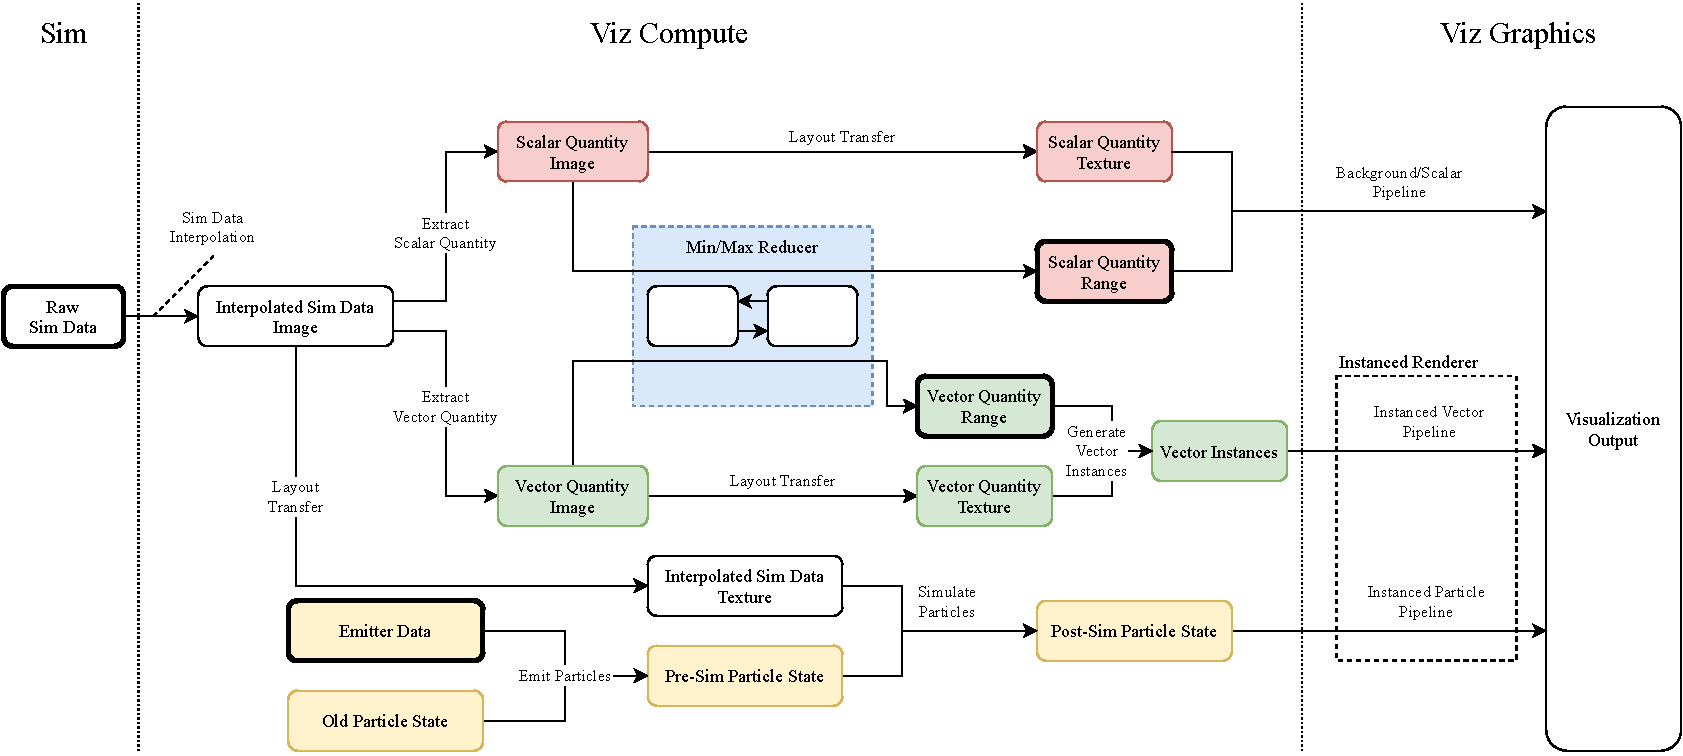
\includegraphics[width=0.9\linewidth]{Ch48Implementation/figures/FinalReport_VizData.pdf}}
    \caption{Data Transformation Diagram showing the data flow for the Visualization}
    \label{fig:VizDataTransform}
\end{sidewaysfigure}
\restoregeometry
\pagebreak
% \end{landscape}

Image layout transfers allow the GPU to optimize access times for an image by changing the format it's stored in.
Images are transferred to the \mintinline{cpp}{ShaderReadOnlyOptimal} layout (listed as `Texture' rather than `Image' in \cref{fig:VizDataTransform}) for efficient sampling at arbitrary points, and kept in the \mintinline{cpp}{General} layout when accessed at 2D data arrays (see \cref{fig:VizImageRead} as a comparison).

Memory barriers (not shown in \cref{fig:VizDataTransform}) are inserted between every compute shader to ensure any required data written from a previous shader is visible to the next shader\cite{TheKhronosGroupVulkanSpec}. % Could also be \cite{MaisterVulkanSyncBlog}
% On top of that, each compute shader requires at least one \emph{memory barrier}, to ensure any data written in previous stages is visible to the next stage.
These memory barriers are quite granular, as shown in \cref{fig:VizMemoryBarrier}.

\begin{figure}
    \centering
     \begin{subfigure}[b]{0.49\textwidth}
         \centering
\begin{glslcode}
uniform readonly image2D resultImage;
 // = (u, v, p, isfluid);

// Specify the exact pixel location
ivec2 pxIdx = ivec2(200, 450);
vec4 data = imageLoad(simDataImage, pxIdx);
\end{glslcode}
\caption{Directly}
        %  \label{fig:vizimageLoad}
     \end{subfigure}
     \hfill
     \begin{subfigure}[b]{0.49\textwidth}
         \centering
\begin{glslcode}
uniform sampler2D simDataSampler;
 // = (u, v, p, isfluid);
 
// 50% across, 20% up the image
vec2 sampleAt = (0.5, 0.2);
vec2 velocity = texture(simDataSampler, sampleAt).xy;
\end{glslcode}
\caption{With a Sampler}
        %  \label{fig:vizimagesample}
     \end{subfigure}
  \caption{Reading from an image directly vs. using a sampler.}
    \label{fig:VizImageRead}
\end{figure}
\begin{figure}
    \centering
    \begin{cppcode}
// Make ShaderWrites from the ComputeShader stage available + visible to 
//      IndirectCommandReads in the DrawIndirect stage
fullMemoryBarrier(computeCmdBuffer,
    vk::PipelineStageFlagBits::eComputeShader, vk::PipelineStageFlagBits::eDrawIndirect,
    vk::AccessFlagBits::eShaderWrite, vk::AccessFlagBits::eIndirectCommandRead);
// Make TransferWrites from the Transfer stage available + visible to the
//      ShaderReads in the ComputeShader phase.
fullMemoryBarrier(computeCmdBuffer,
    vk::PipelineStageFlagBits::eTransfer, vk::PipelineStageFlagBits::eComputeShader,
    vk::AccessFlagBits::eTransferWrite, vk::AccessFlagBits::eShaderRead);
    \end{cppcode}
    \caption{Example showing the granularity of Memory Barriers.}
    \label{fig:VizMemoryBarrier}
\end{figure}

\pagebreak
\begin{figure}[t]
    \centering
    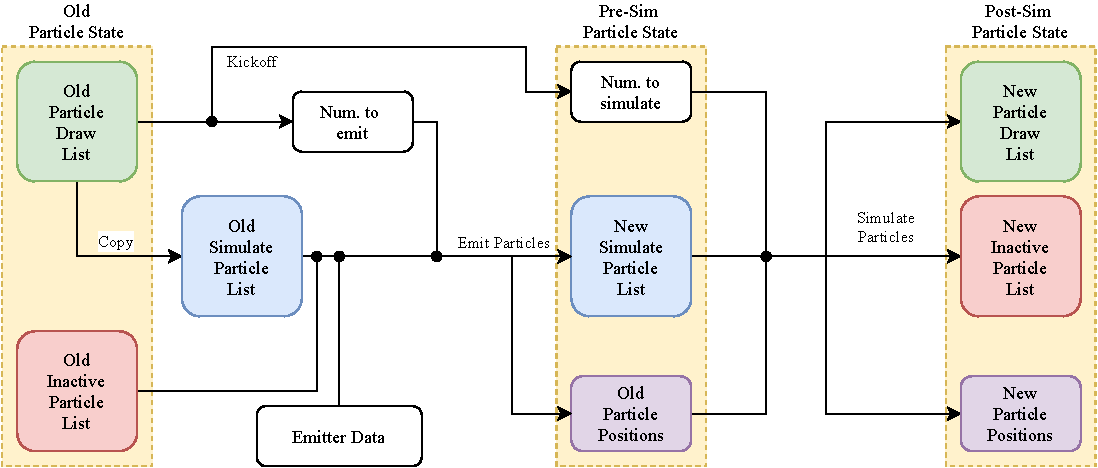
\includegraphics[width=\linewidth]{Ch48Implementation/figures/FinalReport_VizData_Particles.pdf}
    \caption{Breakdown of particle-related GPU work}
    \label{fig:VizDataParticles}
\end{figure}
The particle system implentation in \cref{fig:VizDataTransform} is a simplified view for compactness, \cref{fig:VizDataParticles} shows a full breakdown of this subsystem.
This maintains three growable/shrinkable lists, plus a buffer containing particle positions.
\begin{enumerate}
    \item The Draw list, a list of particle indices to draw on screen
    \item The Inactive list, a list of inactive particle indices
    \item The Simulate list, a list of particle indices which take part in Simulation.
\end{enumerate}
The previous Draw list is the authority on which pariticles currently exist, and is used for the Kickoff shader to determine how many particles will be emitted/simulated\footnote{This isn't known at record time, because the last frame may still be simulating the particles}.
It is also copied into the Simulate particle list, which is grown by the Emit Particles shader.
The particles are then moved by the Simulate Particles shader as shown in \cref{sec:Research:Viz:Particles}.
These particles are added to the inactive list if out-of-bounds, and the new Draw list otherwise.
% adding particles to the inactive list if they move out of the simulation bounds, and moving all other particles to the new Draw list.

\subsection{Safe CPU/GPU Communication}\label{sec:Impl:Viz:CPUGPUSafety}
Unlike CUDA, the Vulkan API does not provide any means of type-safety when communicating between the CPU and GPU.
If the GPU expects data in a specific structure, it is the API user's job to create data that fits this structure.
A naive solution might be to keep a C++ structure definition and a GLSL structure definition, and assume that one matches the other.
This is error prone as the structures are not automatically kept in sync - if one changes, the other will not, and communication will break down.
This project's approach is to create a GLSL file defining all interoperable structures (\texttt{structures.glsl}), and then include it into a C++ header with some extra code to define GLSL types correctly.
Both sides will now use the same structure definitions, which are all defined in exactly one place.
All GLSL code uses the \texttt{std430} memory layout rules, which closely matches the C++ memory layout, so the structures can be passed directly from the CPU to the GPU safely.

\subsection{Usage in Other Layers}
The \mintinline{cpp}{VulkanSimApp} class is instantiated by the command-line layer to run the visualization.

\pagebreak
\section{Command-Line Layer}
The command-line layer is implemented with a set of subapps, each implemented by a separate virtual class satisfying an interface \code{ISubApp}.
Virtual inheritance was chosen here because it is convenient and not in a performance-critical area.
Each ISubApp instance is used to create a CLI11 subcommand with some input arguments, then CLI11 parses the command-line arguments and runs a callback on the selected subapp.
These subapps then invoke other layers of the system to complete their execution.